\section{Methods}

\subsection{Participants}
Twenty participants(10 female, 10 male; all right-handed) from the local university community participated in the experiment. Their age ranged from 21 to 32 years. All participants were naive to the purpose of the experiment and had normal or corrected-to-normal vision. The experiment was approved by the ethics committee of the University of T\"ubingen, and was performed in accordance with the Declaration of Helsinki. Participants gave written informed consent prior to the experiment and were compensated with 8 Euro per hour for their participation. 

\subsection{Apparatus}
The virtual environment was displayed in stereo using an HTC Vive head-mounted-display (HMD) with a resolution of 1080 x 1200 pixels per eye (2160 x 1200 pixels combined). Inter-pupillary distance was measured with a pupilometer and set accoringly on the HTC Vive for each participant. Audio was recorded with a microphone plugged into the integrated audio input of the HTC Vive. Participants were standing during the whole experiment and viewed their virtual task in front of them.

Participants were run in an individual and a collaborative condition in which two participants worked together. Therefore the apparatus consisted of two HTC Vives of which each was connected to its own computer. The computers had the same hardware configuration. In the individual condition participants were run in their own virtual environment solving the task alone. In the collaborative condition two participants were run in a shared virtual environment solving the task together (see Figure \ref{fig:procedure_real_two} and \ref{fig:procedure_vr_two}). The synchronization between the two computers in the collaborative condition was done via UDP. Therefore participants could collaborate in real time with very little to no delay.

The virtual task consists of cubes and cube slots. The cubes can be picked up by moving the controller into a cube and pressing and holding the trigger button of the controller (there is both no collision between cubes and between cubes and the controller). When a cube is picked up it can be moved and rotated freely with the controller. When the cube is moved to the solution space it  automatically aligns ("snaps in") with the next closest cube slot.

\begin{figure}[h]
\centering
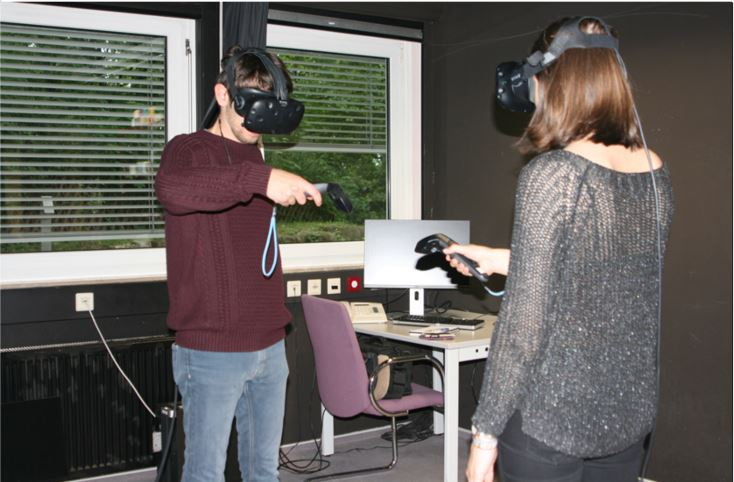
\includegraphics[width=0.75\textwidth]{procedure_real_two}
\caption{Two participants solving the task together in the collaborative condition.} \label{fig:procedure_real_two}
\end{figure}

\begin{figure}[h]
\centering
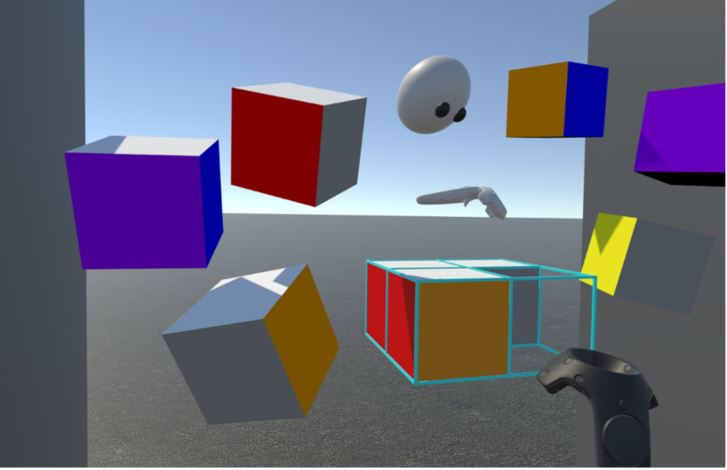
\includegraphics[width=0.75\textwidth]{procedure_vr_two}
\caption{Virtual reality scene of two participants in the collaborative condition. The gray sphere represents the head of the other participant. The gray controller is the controller of the other participant.}
\label{fig:procedure_vr_two}
\end{figure}

\newpage

\subsection{Procedure}
Participants were invited as a group of two people and did not know each other. In one group session the two participants solved the task on their own in a separate virtual environment and together in the same virtual environment. The sequence of single and collaborative condition was counter balanced among all groups. In both the single and collaborative condition participants solved 20 tasks of which all had the same design as described above and differed only in color. In the single condition participants viewed the task always from the same perspective, which means that the starting cube was always placed at the same position in the solution space.
In the collaborative condition we rotated the solution space after 10 trials, which means the starting cube is on one participant's side for the first 10 trials and on the other participant's side for the remaining 10 trials. 

The detailed procedure for the single condition will be explained in the following:
After having read the instructions of the task participants also received a verbal instruction by the experimenter. Before the actual 20 trials began participants had to solve 4 training trials in order to verify that the participant understood the task and the way it has to be solved. It was emphasized that it is important to always stick to the sequence of putting in and removing cubes as described above. Furthermore participants could experience that the starting cube can not be removed and is the only cube in the experiment that collides with the other cubes (that was important to prevent other cubes from overlapping with the starting cube). Participants could also get used to the fact that the top color is always white and the bottom color is always black and that gray always faces to the inside of the solution space. The training trials could be started by the participant by holding a controller button for 2 seconds. When they started the training they saw the solution space surrounded by the 9 cubes which are all in reaching distance. They also saw the starting cube already being placed into the solution space. Above the task participants could see in which trial they currently are. In this case they would see "Training 1/4". Once they have finished a trial they can proceed with the next trial by pressing the controller button again for 2 seconds. 

Before the actual 20 trials started the experimenter repeated the most important instructions. Participants should try to solve the task as quickly and as accurately as possible. Furthermore they were not allowed to move around the problem space and should stay mostly stationary in their position with only a few steps to the sides allowed.
After the 4 training trials participants could start the actual trials as soon as they were ready by clicking a controller button again for 2 seconds. For the actual trial the experimenter would emphasize that participants should always make sure their solution is correct before proceeding with the next task. In case participants did not correctly solve a task and still proceed with the next task the experimenter took notes in order to exclude the trial from the analysis.

The procedure for the collaborative solving of the task was mostly the same. The only difference was that just one participant was able to skip to the next trial and therefore the instructions were that participants had to agree on when to proceed with the next task.

%what needs to go in here is:

%instructions that were given to the participants
%training phase (how many trials...)
%counterbalance single / multi (counterbalanced - 10 each side)
